\section{Framing-based Camera Tool}
GUSTAV

\subsubsection{Keyframing Concept}
Through ?? of Maya we found that the most important feature from here were keyframes.
A keyframe is an event and/or change in one or more parameters over time. Each keyframe corresponds to a point in time, meaning that when the animation reaches this point in time, the values of this keyframe are dominant. Usually this means that in between keyframes some interpolation is happening. This interpolation is per default linear, but can be manipulated in a graph editor. Anything that can be represented by numbers can be manipulated through keyframes.

But games are dynamic, not linear, so this means keyframes can't be associated with a point in time. Specifically for this game, the camera settings would change according to the player's movement, so keyframes needed to be associated with this. Furthermore, the player had to walk on a fixed path, which made the interpolation significantly simpler.

A quick paper prototype of the initial concept showed promise and the idea of associating keyframes with player position was easily understood. To avoid confusion, these keyframes were renamed \textit{framings}. A framing consists of an \textit{influence point} and a camera (see Figure \ref{fig:framingConcept}). When the player's position is the same as an influence point, that framing will dominate, meaning the main camera will use the camera settings of the associated camera. Moving between influence points causes an interpolation between each camera setting. This interpolation can be manipulated in a graph editor, as in Maya.

\begin{figure}[htbp]
\centering
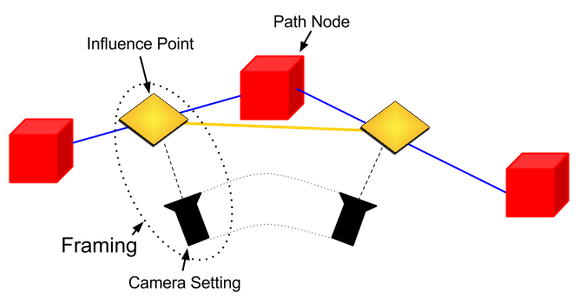
\includegraphics[width=0.4\textwidth]{Pics/Instructions}
\caption{Illustration of the framing concept. A framing consists of an influence point and a group of camera settings.}
\label{fig:framingConcept}
\end{figure}

\subsubsection{Adjusting the Camera}
In Maya, there are multiple ways to accomplish the same thing. An example of this is how to adjust a camera in the scene. This can be done by manually adjusting the X, Y and Z position and rotation of the camera; moving it by dragging a handle tool; or, alternatively, by using the the \textit{Look Through Selected} feature \cite{maya_lookThrough}. During the initial observations, it was clear that many of the artists at The Animation Workshop preferred the latter. This concept was translated directly into the camera tool. Using the \textit{be the camera} feature (see Figure \ref{fig:beTheCam}), the artists can place their camera by navigating the scene in Unity with the \textit{Flythrough mode} \cite{unity_flyMode}.

\begin{figure}[htbp]
\centering
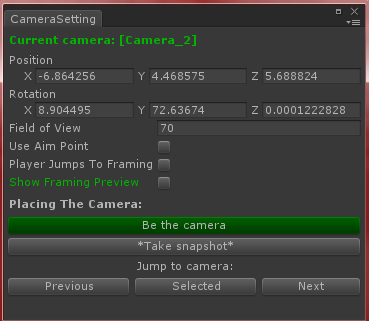
\includegraphics[width=0.3\textwidth]{Pics/be_the_cam_new}
\caption{Pressing the green button puts the user in a special mode where the selected camera inherits position and orientation data from the scene camera. To exit the mode, the user has to press the button again (which at this point shows "Exit the camera" in red).}
\label{fig:beTheCam}
\end{figure}

Another way to adjust the camera in Maya is by using an aim-vector control point \cite{maya_camAim}. The artists at The Animation Workshop used this to quickly make the camera aim at something in the scene. This concept has also been designed for the camera tool (see Figure \ref{fig:aimPoint}).

\begin{figure}[htbp]
\centering
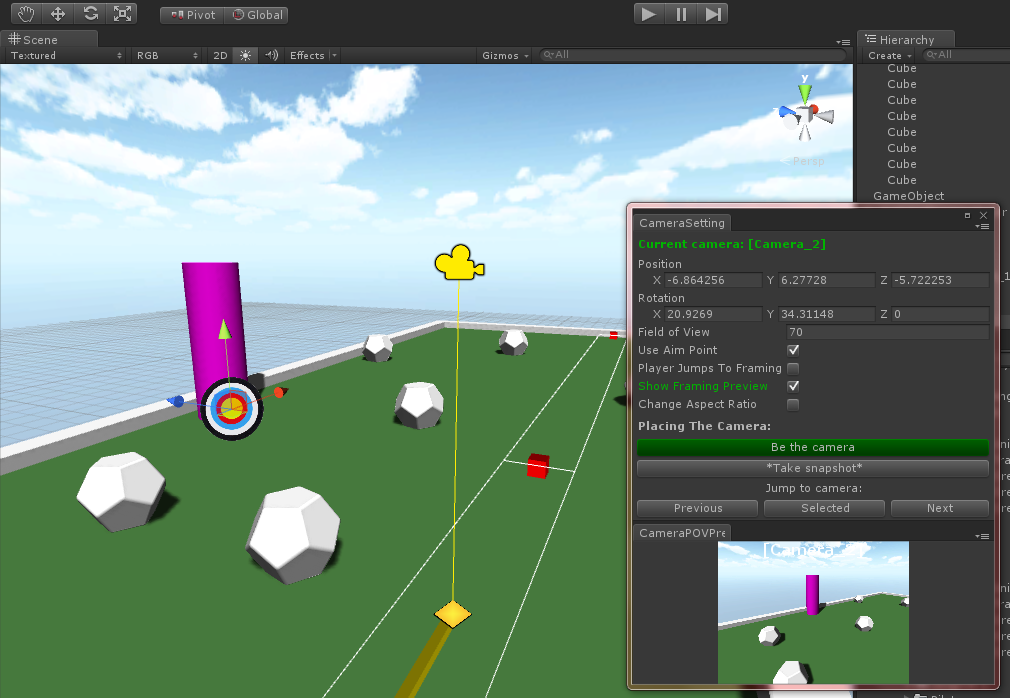
\includegraphics[width=0.3\textwidth]{Pics/aimPoint}
\caption{The aim point allows for quick adjustments of the camera.}
\label{fig:aimPoint}
\end{figure}

%It was discovered that none of the artists knew how to use a standard Unity feature that lets the player fly around with the scene camera as if they were playing a first-person game ("Flythrough Mode", \cite{unity_flyMode}). The artist were excited about the discovery of this feature. One artist perceived the standard way of moving around in Unity as confusing, while another stated that the way of moving the camera is exactly like in Maya. After testing this ourselves, we concluded that the movement controls in Maya and Unity are indeed very similar (except for the "Flythrough Mode"), which means that the artists should ideally be comfortable with navigating in either of the applications.

\subsubsection{Immediate Feedback \& Quick Preview}
%An important aspect for the tool was to provide clear feedback.
A common request from all of the artists were the ability to quickly preview their changes. Instead of having to start the game and navigate the player character to a specific framing, the artists wanted to quickly jump to a specific framing to test out how it feels and looks.

The artists suggested that they should be able to move the player character around in the editor. Initially, this seemed like a fine way to preview the framings. We did design this feature, but deemed it a bit impractical, since it sometimes would be hard to locate the player character in a big scene. Instead, we took inspiration from Camera Path Animator 3.0 mentioned in Section \ref{relatedWork} by designing an interactive slider. With this feature, the artists are able to choose the start and end framing and interpolate between these. By dragging the slider between those, the artists can quickly get a feel of how the camera movements will look (see Figure \ref{fig:slider}). Alternatively, they can press a "play" button to preview the interpolation and get a feel of the actual player velocity.

\begin{figure}[htbp]
\centering
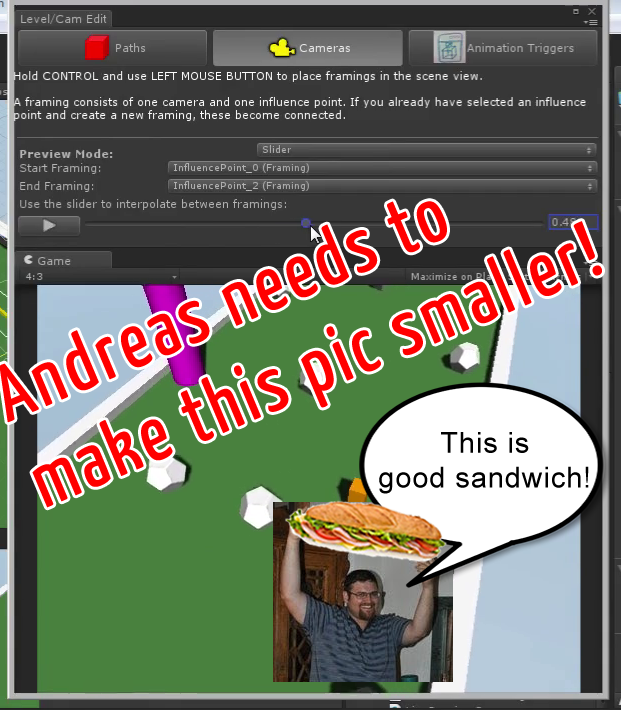
\includegraphics[width=0.3\textwidth]{Pics/slider}
\caption{The slider provides a quick way to preview the framings.}
\label{fig:slider}
\end{figure}

%\subsection{Participatory Design Conclusion}
%It's important to design and iterate with the users' current workflow and mental models in mind. By building on top of their pre-exisiting skills and knowledge, one can ease the learning curve by creating a design that is close to what the users are already familiar with. The users should become co-creators, but you should not forget that \textit{you} are the designer. You should listen to what the users say they want, but even more so try to understand what they really \textit{need} and \textit{why} they need it.